%!TEX root = main.tex


\section{Probability with connectable submodels}

Throughout this paper, we will assume all measurable sets $X$ are finite sets. This is both because it makes explanations simpler and because it is easy to show that submodels exist in this setting (Lemma \ref{lem:subm_exist}). Many of the proofs in this paper can likely be specialised to more general settings due to our use of string diagrams which represent abstract morphisms in Markov categories, rather than finite Markov kernels specifically.

The standard method of constructing probability models introduces a probability space $(\prob{P},(\Omega,\sigalg{F}))$ with $\Omega$ a sample space, $\sigalg{F}$ a $\sigma$-algebra on $\Omega$ and $\prob{P}$ a probability measure on $(\Omega,\sigalg{F})$. Random variables are defined by measurable functions on $\Omega$ and are given names in sans-serif like $\RV{X}$. A probability distribution $\prob{P}^{\RV{XYZ}}$ is ``the joint distribution of $\RV{X}$, $\RV{Y}$ and $\RV{Z}$ under $\prob{P}$'' where $\RV{X},$ $\RV{Y}$ and $\RV{Z}$ are associated with random variables on $\Omega$ and is given by the pushforward of the function $\omega\mapsto (\RV{X}(\omega),\RV{Y}(\omega),\RV{Z}(\omega))$. Unless otherwise stated, a random variable named $\RV{X}$ will take values in the space $X$ (note the serif font).

We want to consider an extension of this approach for reasoning about causal modelling. The causal graphical models literature provides some simple examples illustrating this need, while the fact that the potential outcomes approach also benefits from extension requires more explanation, and will be discussed in Section \ref{sec:potential_outcomes}. 

Consider the ``truncated factorisation'', a linchpin operation in causal graphical models. Given a probability $\prob{P}^{\RV{XYZ}}$ and the assumption that the results of interventions are described by $\prob{P}$ along with a graphical model in which $\RV{Z}$ blocks all backdoor paths between $\RV{X}$ and $\RV{Y}$, we can define a new probability measure $\prob{P}_x$ representing the result of ``setting $\RV{X}$ to $x$'' by truncated factorisation \citep[page ~24]{pearl_causality:_2009}:
\begin{align}
	\prob{P}^{\RV{XYZ}}_{x}(x',y,z):=\prob{P}^{\RV{Y|XZ}}(y|x,z)\prob{P}^{\RV{Z}}(z)\llbracket x=x'\rrbracket\label{eq:truncated_fac}
\end{align}

Without a causal model justifying the claim that $\RV{Z}$ blocks backdoor paths between $\RV{X}$ and $\RV{Y}$, there is in general no special siginificance to the expression on the right side of Equation \ref{eq:truncated_fac}, and causal models that can justify such claims are not a feature of the standard approach to probability modelling. At the same time, the notation we have chosen for the left side of Equation \ref{eq:truncated_fac} suggests that $\prob{P}^{\RV{XYZ}}_{x}$ is a distribution over the same variables $\RV{X}$, $\RV{Y}$ and $\RV{Z}$ as the original $\prob{P}^{\RV{XYZ}}$. The standard approach to probability modelling \emph{does} offer an account of what it means for variables to be the same, which is that they are represented by the same measurable functions on the probability space.

An immediate issue is that $\prob{P}_x$ is a different probability measure to $\prob{P}$. However, even if we substitute probability measures, we could perhaps keep the sample space $\Omega$ and define variables as measurable functions on $\Omega$. This is the approach taken in \citet{pearl_causality:_2009} (but see Section \ref{sec:vague_variables}).

This rules out the possibility of performing some interventions. For example, if $\RV{X}=\RV{Z}$ and $\RV{X}$ can take more than one value, then no $\prob{P}_x$ exists with the property required by Equation \ref{eq:truncated_fac}.

For an example of an intervention we \emph{want} to rule out, consider a variable $\RV{B}$ representing a person's body mass index. It seems reasonable to hold that this variable is by definition equivalent to $\frac{\RV{W}}{\RV{H}^2}$ where $\RV{W}$ represents their weight in kilograms and $\RV{H}$ represents their height in metres. This rules out the existence of any probability measure that represents the results of an intervention on $\RV{B}$ in any model that also contains $\RV{H}$ and $\RV{W}$ and features the expected causal relationships (and, regardless of causal relationships, it completely rules out the possibility that $\RV{B}$, $\RV{H}$ and $\RV{W}$ can all be intervened on). Such interventions can be ruled out by defining the random variables such that $\RV{B} = \frac{\RV{W}}{\RV{H}^2}$.

Along the same lines as \citet{dawid_causal_2000}, we find that it is often desirable to introduce variables representing the results of choices, and we often don't want to attach probability distributions to such variables. We might have $\RV{D}$, representing a choice, and $\prob{P}^{\RV{Y}|\RV{D}}$ representing the consequences of this choice, but no $\prob{P}^{\RV{Y},\RV{D}}$ as we have no need of a marginal probability of $\RV{D}$.

As a brief summary, we want a version of ``probability theory'' that:
\begin{itemize}
	\item Defines what we mean by a ``variable''
	\item Includes generalised variables that do not have marginal probabilities (for example, to represent choices)
	\item Can express operations like Equation \ref{eq:truncated_fac}
\end{itemize}

Standard probability theory does the first, but not the second two. 

\subsection{Markov categories}
We base our approach on the theory of Markov categories. This has two benefits: firstly, Markov categories have a graphical notation that help present some ideas in an intuitive manner. Secondly, because they are abstract categories that represent models of the flow of information, proofs that use only string diagrams correspond to theorems in many formalisations of probability, not just the finite set case that we focus on here. More comprehensive introductions to Markov categories can be found in \citet{fritz_synthetic_2020,cho_disintegration_2019}.

Rather than explain Markov categories in the abstract, we will instead introduce string diagrams with reference to how they represent stochastic maps and finite sets (though see Appendix \ref{sec:app_mcat}). Given measurable sets $(X,\sigalg{X})$ and $(Y,\sigalg{Y})$, a Markov kernel or stochastic map is a map $\kernel{K}:X\times \sigalg{Y}\to [0,1]$ such that

\begin{itemize}
	\item The map $x\mapsto \kernel{K}(x,A)$ is $\sigalg{X}$-measurable for every $A\in \sigalg{Y}$
	\item The map $A\mapsto \kernel{K}(x,A)$ is a probability measure for every $x\in X$
\end{itemize}

Where $X$ and $Y$ are finite sets with the discrete $\sigma$-algebra, we can represent a Markov kernel $\kernel{K}$ as a $|X|\times |Y|$ matrix where $\sum_{y\in Y} \kernel{K}_x^y = 1$ for every $x\in X$. We will give Markov kernels the signature $\kernel{K}:X\kto Y$ to indicate that they map from $X$ to probability distributions on $Y$.

Graphically, Markov kernels are drawn as boxes with input and output wires, and probability measures (which are kernels with the domain $\{*\}$) are represented by triangles:

\begin{align}
\kernel{K}&:=\begin{tikzpicture}[baseline={([yshift=-.5ex]current bounding box.center)}]
	\path (0,0) node (A) {}
	++ (0.5,0) node[kernel] (K) {$\kernel{K}$}
	++ (0.5,0) node (B) {};
	\draw (A) -- (K) -- (B);
\end{tikzpicture}\\
\kernel{P}&:= \begin{tikzpicture}[baseline={([yshift=-.5ex]current bounding box.center)}]
	\path (0,0) node[dist] (K) {$\kernel{P}$}
	++ (0.5,0) node (B) {};
	\draw (K) -- (B);
\end{tikzpicture}
\end{align}

Two Markov kernels $\kernel{L}:X\kto Y$ and $\kernel{M}:Y\kto Z$ have a product $\kernel{L}\kernel{M}:X\kto Z$ given by the matrix product $\kernel{L}\kernel{M}_x^z = \sum_y \kernel{L}_x^y\kernel{M}_y^z$. Graphically, we write represent by joining wires together:

\begin{align}
	\kernel{L}\kernel{M}:= \begin{tikzpicture}[baseline={([yshift=-.5ex]current bounding box.center)}]
	\path (0,0) node (A) {}
	++ (0.5,0) node[kernel] (K) {$\kernel{K}$}
	++ (0.7,0) node[kernel] (M) {$\kernel{M}$}
	++ (0.5,0) node (B) {};
	\draw (A) -- (K) -- (M) -- (B);
\end{tikzpicture}
\end{align}

The Cartesian product $X\times Y:=\{(x,y)|x\in X, y\in Y\}$. Given kernels $\kernel{K}:W\kto Y$ and $\kernel{L}:X\kto Z$, the tensor product $\kernel{K}\otimes\kernel{L}:W\times X\kto Y\times Z$ is defined by $(\kernel{K}\otimes\kernel{L})_{(w,x)}^{(y,z)}:=K_{w}^y L_{x}^z$ and represents applying the kernels in parallel to their inputs.

The tensor product is represeted by drawing kernels in parallel:

\begin{align}
	\kernel{K}\otimes \kernel{L}&:=\begin{tikzpicture}[baseline={([yshift=-.5ex]current bounding box.center)}]
	\path (0,0) node (A) {$W$}
	++ (0.5,0) node[kernel] (K) {$\kernel{K}$}
	++ (0.5,0) node (B) {$Y$};
	\path (0,-0.5) node (C) {$X$}
	++ (0.5,0) node[kernel] (L) {$\kernel{L}$}
	++ (0.5,0) node (D) {$Z$};
	\draw (A) -- (K) -- (B);
	\draw (C) -- (L) -- (D);
\end{tikzpicture}
\end{align}

We read diagrams from left to right (this is somewhat different to \citet{fritz_synthetic_2020,cho_disintegration_2019,fong_causal_2013} but in line with \citet{selinger_survey_2010}). A diagram describes products and tensor products of Markov kernels, which are expressed according to the conventions described above. There are a collection of special Markov kernels for which we can replace the generic ``box'' of a Markov kernel with a diagrammatic elements that are visually suggestive of what these kernels accomplish.

A description of these kernels follows.

The identity map $\text{id}_X:X\kto X$ defined by $(\text{id}_X)_x^{x'}= \llbracket x = x' \rrbracket$, where the iverson bracket $\llbracket \cdot \rrbracket$ evaluates to $1$ if $\cdot$ is true and $0$ otherwise, is a bare line:

\begin{align}
	\mathrm{id}_X&:=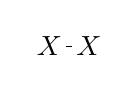
\begin{tikzpicture}[baseline={([yshift=-.5ex]current bounding box.center)}]
	\path (0,0) node (A) {$X$} ++ (0.5,0) node (B) {$X$};
	\draw (A) -- (B);
\end{tikzpicture}
\end{align}

We choose a particular 1-element set $\{*\}$ that acts as the identity in the sense that $\{*\}\times A=A\times \{*\} = A$ for any set $A$. The erase map $\text{del}_X:X\kto \{*\}$ defined by $(\text{del}_X)_x^* = 1$ is a Markov kernel that ``discards the input'' (we will later use it for marginalising joint distributions). It is drawn as a fuse:

\begin{align}
	\text{del}_X&:=\begin{tikzpicture}[baseline={([yshift=-.5ex]current bounding box.center)}]
	\path (0,0) ++ (1,0) node (B) {$X$};
	\draw[-{Rays[n=8]}] (A) -- (B);
\end{tikzpicture}
\end{align}

The copy map $\text{copy}_X:X\kto X\times X$ defined by $(\text{copy}_X)_x^{x',x''}=\llbracket x=x' \rrbracket \llbracket x=x'' \rrbracket$ is a Markov kernel that makes two identical copies of the input. It is drawn as a fork:

\begin{align}
	\text{copy}_X&:=\begin{tikzpicture}[baseline={([yshift=-.5ex]current bounding box.center)}]
	\path (0,0) node (A) {$X$} 
	++ (0.5,0) node[copymap] (copy0) {}
	++ (0.5,0.15) node (B) {$X$}
	+ (0,-0.3) node (C) {$X$};
	\draw (A) -- (copy0) to [out=45,in=180] (B) (copy0) to [out=-45, in=180] (C);
\end{tikzpicture}
\end{align}

The swap map $\text{swap}_{X,Y}:X\times Y\kto Y\times X$ defined by $(\text{swap}_{X,Y})_{x,y}^{y',x'}=\llbracket x=x' \rrbracket\llbracket y=y' \rrbracket$ swaps two inputs, and is represented by crossing wires:

\begin{align}
	\text{swap}_X &:=  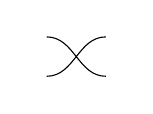
\begin{tikzpicture}[baseline={([yshift=-.5ex]current bounding box.center)}]
		\path (0,0) node (A) {} 
		+ (0,-0.5) node (B) {}
		++ (1,0) node (C) {}
		+ (0,-0.5) node (D) {};
		\draw (A) to [out=0,in=180] (D) (B) to [out=0, in=180] (C);
	\end{tikzpicture}
\end{align}

Because we anticipate that the graphical notation will be unfamiliar to many, we will also include translations to more familiar notation.

\subsection{Truncated factorisation with Markov kernels}

The Markov kernels introduced in the previous section can be though of as ``conditional probability distributions without variables''. We can use these to represent an operation very similar to Equation \ref{eq:truncated_fac}. Note that $P^{\RV{Y|XZ}}$ must be represented by a Markov kernel $\kernel{K}:X\times Z\kto Y$ and $\prob{P}^{\RV{Z}}$ by a Markov kernel $\kernel{L}\in \Delta(Z)$. Then we can define a Markov kernel $\kernel{M}:X\kto X\times Z$ representing $x\mapsto \prob{P}^{\RV{YZ}}_{x}(y,z)$ by

\begin{align}
	\kernel{M}:= \tikzfig{truncated_factorisation}\label{eq:tfac_setted}
\end{align}

There is, however, a key difference between Equation \ref{eq:tfac_setted} and Equation \ref{eq:truncated_fac}: the Markov kernels in the latter equation describe the distribution of particular variables, while the former equation describes Markov kernels only.

To illustrate why we need variables, consider an arbitrary Markov kernel $\kernel{K}:\{*\}\kto \Delta(X\times X)$. We could draw this:
\begin{align}
	\kernel{K}:= \tikzfig{double_label}\label{eq:double_label}
\end{align}
We label both wires with the set $X$. However, say $X=\{0,1\}$. Then $\kernel{K}$ could be the kernel $\kernel{K}^{x_1,x_2} = \llbracket x_1 = 0\rrbracket \llbracket x_2 = 1\rrbracket$. In this case, both of its outputs must represent \emph{different} variables, despite taking values in the same set. On the other hand, if $\kernel{K}^{x_1,x_2} = 0.5 \llbracket x_1 = x_2 \rrbracket$ then both outputs coudl represent the same variable, because they are deterministically the same, or they could represent different variables that happen to be equal. We need some way to distinguish the two cases.

We use a definition of variable that almost matches the standard definition we introduced at the beginning of the section. We define variables as Markov kernels rather than functions as it makes the construction slightly simpler.

\begin{definition}[Variable]
Given a \emph{sample space} $\Omega$, a variable $\RV{X}$ is a Markov kernel $\Omega\kto A$ such that there exists some function $f_{\RV{X}}:\Omega\to A$
with $\RV{X}_x^a=\llbracket a = f_{\RV{X}}(x) \rrbracket$.
\end{definition}

We define the \emph{product} of two variables as follows:
\begin{itemize}
	\item \textbf{Product:} Given variables $\RV{W}:\Omega\kto A$ and $\RV{V}:\Omega\kto B$, the product is defined as $(\RV{W}, \RV{V})=\text{copy}_{\Omega} (\RV{W}\otimes\RV{V})$
\end{itemize}

The \emph{unit} variable is the erase map $\RV{I}:=\text{del}_\Omega$, with $(\RV{I},\RV{X})=(\RV{X},\RV{I})=\RV{X}$ (up to isomorphism) for any $\RV{X}$.

We then need a notion of Markov kernels that ``maps between variables''. An \emph{indexed Markov kernel} is such a thing.

\begin{definition}[Indexed Markov kernel]
Given variables $\RV{X}:\Omega\to A$ and $\RV{Y}:\Omega\to B$, an indexed Markov kernel $\kernel{K}:\RV{X}\kto \RV{Y}$ is a triple $(\kernel{K}',\RV{X},\RV{Y})$ where $\kernel{K}':A\kto B$ is the \emph{underlying kernel}, $\RV{X}$ is the \emph{input index} and $\RV{Y}$ is the \emph{output index}.
\end{definition}

For example, if $\kernel{K}:(\RV{A}_1,\RV{A}_2)\to \Delta(\RV{B}_1,\RV{B}_2)$, for example, we can draw:

\begin{align}
	\kernel{K} := \begin{tikzpicture}[baseline={([yshift=-.5ex]current bounding box.center)}]
	\path (0,0) node (A1) {$\RV{A}_1$}
	+ (0,-0.3) node (A2) {$\RV{A}_2$}
	++ (0.7,-0.15) node[kernel] (K) {$\kernel{K}$}
	++ (0.7,0.15) node (B1) {$\RV{B}_1$}
	+ (0,-0.3) node (B2) {$\RV{B}_2$};
	\draw (A1) -- ($(K.west) + (0,0.15)$) (A2) -- ($(K.west) + (0,-0.15)$);
	\draw (B1) -- ($(K.east) + (0,0.15)$) (B2) -- ($(K.east) + (0,-0.15)$);
\end{tikzpicture}
\end{align}

or

\begin{align}
	\kernel{K} = \begin{tikzpicture}[baseline={([yshift=-.5ex]current bounding box.center)}]
	\path (0,0) node (A1) {$(\RV{A}_1,\RV{A}_2)$}
	++ (1.3,0) node[kernel] (K) {$\kernel{K}[\model{L}]$}
	++ (1.3,0.) node (B1) {$(\RV{B}_1,\RV{B}_2)$};
	\draw (A1) -- (K) -- (B1);
\end{tikzpicture}
\end{align}

We define the product of indexed Markov kenrnels $\kernel{K}:\RV{X}\kto \RV{Y}$ and $\kernel{L}:\RV{Y}\kto \RV{Z}$ as the triple $\kernel{K}\kernel{L}:=(\kernel{K}'\kernel{L}',\RV{X},\RV{Z})$.

Similarly, the tensor product of $\kernel{K}:\RV{X}\kto\RV{Y}$ and $\kernel{L}:\RV{W}\kto\RV{Z}$ is the triple $\kernel{K}\otimes\kernel{L}:=(\kernel{K}'\otimes\kernel{L}',(\RV{X},\RV{W}),(\RV{Y},\RV{Z}))$.

We define $\text{Id}_{\RV{X}}$ to be the model $(\text{Id}_X,\RV{X},\RV{X})$, and similarly the indexed versions $\text{del}_{\RV{X}}$, $\text{copy}_{\RV{X}}$ and $\text{swap}_{\RV{X},\RV{Y}}$ are obtained by taking the unindexed versions of these maps and attaching the appropriate random variables as indices. Diagrams are the diagrams associated with the underlying kernel, with input and output wires annotated with input and output indices.

The category of indexed Markov kernels as morphisms and variables as objects is a Markov category (Appendix \ref{sec:app_mcat}), and so a valid derivation based on the string diagram language for Markov categories corresponds to a valid theorem in this category. However, most of the diagrams we can form are not viable candidates for models of our variables. For example, if $\RV{X}$ takes values in $\{0,1\}$ we can propose an indexed Markov kernel $\kernel{K}:\RV{X}\kto\RV{X}$ with $\kernel{K}'_x^{x'}=0.5$ for all $x, x'$. However, this is not a viable model of the variable $\RV{X}$, because it expresses something like ``if we know the value of $\RV{X}$, then we belive that $\RV{X}$ could take any value with equal probability''.

We define a \emph{model} as ``an indexed Markov kernel that assigns probability 0 to things known to be contradictions''.

\begin{definition}[Model]
An indexed Markov kernel $(\kernel{K}',\RV{X},\RV{Y})$ is a \emph{model} if it assigns probability 0 to contradictions. That is:
\begin{align}
	\max_{\omega\in \Omega} (\RV{X},\RV{Y})_{\omega}^{a,b} = 0 \implies \left(\kernel{K}_{a}^{\prime b} = 0\right) \lor \left(\max_{\omega\in \Omega} \RV{X}_{\omega}^{a} = 0\right)
\end{align}
A \emph{probability model} is a model where the underlying kernel $\kernel{K}'$ has the unit $\RV{I}$ as the domain. We use the font $\model{K}$ to distinguish models from arbitrary indexed Markov kernels.
\end{definition}

We can think of $\RV{X}$ as the antecedent and $\RV{Y}$ as the consequent in this definition. If there is no $\omega$ such that $f_{\RV{X}}(\omega)=a$, no restrictions are applied (from a contradiction, one may conclude anything). If there is no $\omega\in \Omega$ such that $f_\RV{X}(\omega)=a$ and $f_\RV{Y}(\omega)={b'}$ then the probability of $\RV{Y}=b$ when $\RV{X}=a$ must be zero. If $f_{\RV{X}}(\omega)=a\implies f_{\RV{Y}}(\omega)=b$ then the probability of $\RV{Y}=b$ when $\RV{X}=a$ must be one (because 0 probability must be assigned to all other pairs of values).

Non-contradiction implies that for any $\RV{X}:\Omega\kto A$, there is a unique model mapping $\text{Id}_\Omega$ to $\RV{X}$ for which the underlying kernel is $\RV{X}$ itself (Lemma \ref{lem:uniq_model}). One consequence of this is, given a probability model of the sample space $\model{P}:\RV{I}\kto \text{Id}_\Omega$ (``a probability measure on $\Omega$''), $\model{P}\RV{X}$ is the unique measure on $\RV{X}$ obtainable by composition of a model with $\prob{P}$. $\model{P}\RV{X}$ is the pushforward of $\model{P}$ by $\RV{X}$. That is, non-contradiction implies that, given a probability model of the sample space, there is a unique corresponding probability model of $\RV{X}$ is given by the pushforward of $\RV{X}$ (corollary \ref{corr:pushforward}).

\begin{lemma}[Uniqueness of models with the sample space as a domain]\label{lem:uniq_model}
For any $\RV{X}:\Omega\to A$, there is a unique model $\model{X}:\text{Id}_\Omega\kto \RV{X}$ given by $\model{X}:=(\RV{X},\text{Id}_\Omega,\RV{X})$.
\end{lemma}

\begin{proof}
$\RV{X}$ is a Markov kernel mapping from $\Omega\to A$, so it is a valid underlying kernel for $\model{X}$, and $\model{X}$ has input and output indices matching its signature. We need to show it satisfies non-contradiction.

For any $\omega\in \Omega$, $a\in A$
\begin{align}
	\max_{\omega\in \Omega}(\text{Id}_\Omega,\RV{X})_{\omega}^{\omega',a} &= \max_{\omega\in \Omega} \llbracket \omega = \omega' \rrbracket \llbracket \omega = f_{\RV{X}}(a) \rrbracket\\
	&= \llbracket \omega = f_{\RV{X}}(a) \rrbracket\\
	&= \kernel{X}_\omega^a
\end{align}
Thus $\model{X}$ satisfies non-contradiction.

Suppose there were some $\model{K}:\text{Id}_\Omega\kto \RV{X}$ not equal to $\RV{X}$. Then there must be some $\omega\in \Omega$, $b\in A$ such that $\model{K}_\omega^b\neq 0$ and $f_{\RV{X}}(\omega)\neq b$. Then
\begin{align}
	\max_{\omega\in \Omega}(\text{Id}_\Omega,\RV{X})_{\omega}^{\omega',a} &= \max_{\omega\in \Omega} \llbracket \omega = \omega' \rrbracket \llbracket \omega = f_{\RV{X}}(b) \rrbracket\\
	&= \llbracket \omega = f_{\RV{X}}(b) \rrbracket\\
	&= 0\\
	&< \model{K}_\omega^b
\end{align}
Thus $\model{K}$ doesn't satisfy non-contradiction.
\end{proof}

\begin{corollary}[Pushforward measure]\label{corr:pushforward}
Given any probability model $\model{P}:\RV{I}\kto \text{Id}_\Omega$, there is a unique probability model $\model{P}^{\RV{X}}:\RV{I}\kto \RV{X}$ such that $\model{P}^{\RV{X}}=\model{P}\model{Q}$ for some $\model{Q}:\text{Id}_\Omega\to \RV{X}$ and it is given by $(\model{P}^{\RV{X}})^a = \sum_{\omega\in f^{-1}(a)} \model{P}^{\omega}$.
\end{corollary}

\begin{proof}
As $\model{X}:=(\RV{X},\text{Id}_\Omega,\RV{X})$ is the unique model $\text{Id}_\Omega\to \RV{X}$, it must be the case that $\model{P}^{\RV{X}}=\model{P}\model{X}$. Then for any $a\in A$
\begin{align}
	(\model{P}\model{X})^a &= \sum_{\omega\in \Omega} \model{P}^\omega\RV{X}_\omega^a\\
						 &= \sum_{\omega\in \Omega} \model{P}^\omega \llbracket a = f_{\RV{X}}(\omega) \rrbracket\\
						 &= \sum_{\omega\in f^{-1}(a)} \model{P}^{\omega}
\end{align}
\end{proof}

We also show a number of other useful properties. 

\begin{lemma}[Output copies of the same variable are identical]\label{lem:nocopy1}
If $\model{K}:\RV{X}\kto (\RV{Y},\RV{Y},\RV{Z})$ is a model, there exists some $\model{L}:\RV{X}\kto (\RV{Y},\RV{Z})$ such that
\begin{align}
		\model{K}_{x}^{\prime y,y',z} &= \llbracket y=y' \rrbracket\model{L}_{x}^{\prime y,z}\\
\end{align}
\end{lemma}

\begin{proof}
For any $\omega,x,y,y',z$:
\begin{align}
	(\RV{X},\RV{Y},\RV{Y},\RV{Z})_\omega^{x,y,y',z} &= \llbracket f_{\RV{Y}}(\omega)=y \rrbracket \llbracket f_{\RV{Y}}(\omega)=y' \rrbracket (\RV{X},\RV{Z})_\omega^{x,z} \\
	&= \llbracket y=y' \rrbracket \llbracket f_{\RV{Y}}(\omega)=y \rrbracket(\RV{X},\RV{Z})_\omega^{x,z}
\end{align}
Therefore, by non-contradiction, for any $x,y,y',z$, $y\neq y'\implies \model{K}_{x}^{\prime yy'z}=0$. Define $\model{L}$ by $\model{L}_x^{\prime y, z} := \model{K}_x^{\prime y y z}$. The fact that $\model{L}$ is a model follows from the assumption that $\model{K}$ is. Then
\begin{align}
	\model{K}_{x}^{\prime y,y',z} &= \llbracket y=y' \rrbracket\model{L}_{x}^{\prime y,z}
\end{align}
\end{proof}


\begin{lemma}[Copies shared between input and output are identical]\label{lem:nocopy2}
For any $\model{K}:(\RV{X},\RV{Y})\kto (\RV{X},\RV{Z})$, there exists some $\model{L}:(\RV{X},\RV{Y})\kto \RV{Z}$ such
\begin{align}
	 \model{K}_{x,y}^{\prime x',z} &= \llbracket x=x'\rrbracket \model{L}_{\prime x,y}^{z}
\end{align}
\end{lemma}

\begin{proof}
For any $\omega,x,y,y',z$:
\begin{align}
	(\RV{X},\RV{Y},\RV{Y},\RV{Z})_\omega^{x,y,y',z} &= \llbracket f_{\RV{Y}}(\omega)=y \rrbracket \llbracket f_{\RV{Y}}(\omega)=y' \rrbracket (\RV{X},\RV{Z})_\omega^{x,z} \\
	&= \llbracket y=y' \rrbracket \llbracket f_{\RV{Y}}(\omega)=y \rrbracket(\RV{X},\RV{Z})_\omega^{x,z}
\end{align}
Therefore, by non-contradiction, for any $x,y,y',z$, $x\neq x'\implies \model{K}_{x,y}^{\prime x'z}=0$. Define $\model{L}$ by $\model{L}_{x,y}^{\prime x', z} := \model{K}_{x,y}^{\prime x, y}$. The fact that $\model{L}$ is a model again follows from the assumption that $\model{K}$ is a model. Then
\begin{align}
	\model{K}_{x, y}^{\prime x', z} &= \llbracket x=x' \rrbracket\model{L}_{x,y}^{\prime z}
\end{align}
\end{proof}

\subsection{Truncated factorisation a third time}

At this point, we can represent Equation \ref{eq:truncated_fac} using models. Suppose $P^{\RV{Y|XZ}}$ is an model $\model{K}:(\RV{X}, \RV{Z})\kto \RV{Y}$ and $\prob{P}^{\RV{Z}}$ an model $\model{L}:\{*\}\kto \RV{Z}$. Then we can define an indexed Markov kernel $\kernel{M}:\RV{X}\kto \RV{X}, \RV{Z}$ representing $x\mapsto \prob{P}^{\RV{YZ}}_{x}(y,z)$ by

\begin{align}
	\kernel{M}&:= \tikzfig{truncated_factorisation_labeled}\label{eq:tfac_labeled}
\end{align}

Equation \ref{eq:tfac_labeled} is almost identical to Equation \ref{eq:tfac_setted}, except it now specifies which variables each measure applies to, not just which sets they take values in. Like the original Equation \ref{eq:truncated_fac}, there is no guarantee that $\kernel{M}$ is actually a model. If $f_\RV{X}=g\circ f_\RV{Z}$ for some $g:Z\to X$ and $X$ has more than 1 element, then the rule of non-contradiction will rule out the existence of any such model.

We don't know an easy way to check whether an arbitrary construction like Equation \ref{eq:tfac_labeled} is a model. 

Instead, we will 

\subsection{Submodels}

We do not yet have a notion of \emph{marginal probability} or \emph{conditional probability}. In the paragraph above, the terms $P^{\RV{Y|XZ}}$ and $P^{\RV{Z}}$ are external to the theory we have postulated so far. In particular, the idea that $P^{\RV{Y|XZ}}$ and $P^{\RV{Z}}$ are both parts of a larger model $P$ is not something we can yet express. We will use the term \emph{submodels} to refer to marginals and conditionals of a larger model.

\begin{definition}[Marginalising model]
For any variable $\RV{X}:\Omega\to A$, a model $\kernel{K}:\RV{Y}\kto \RV{Z}$ \emph{marginalises over} $\RV{X}$ if there exists some $\RV{W}$ such that $\RV{Y}=(\RV{X},\RV{W})$ and $\kernel{K}=\text{del}_{\RV{X}}\otimes \text{Id}_{\RV{W}}$.
\end{definition}

Note that any model $\kernel{M}:\RV{Y}\kto\RV{Z}$ that marginalises over $*$ is equal to $\text{del}_*\otimes \text{Id}_{\RV{Y}}=\text{Id}_{\RV{Y}}$.

\begin{definition}[Marginal submodel]\label{def:marg_submodel}
Given any $\kernel{K}:\RV{X}\kto\RV{Y}$, any $\kernel{L}:\RV{X}\kto\RV{Z}$ and any variable $\RV{A}$, $\kernel{L}$ is a \emph{marginal submodel} of $\kernel{K}$ if there is some model $\kernel{M}:\RV{Y}\kto \RV{Z}$ that marginalises over $\RV{A}$ such that $\kernel{L}=\kernel{KM}$.
\end{definition}

Because $\kernel{K} \text{Id}_{\RV{Y}}=\kernel{K}$, and $\text{Id}_{\RV{Y}}$ is the model that marginalises over $*$, $\kernel{K}$ is always a marginal of itself.

\begin{definition}[Conditional submodel]\label{def:submodel}
Given $\kernel{K}:\RV{X}\kto \RV{Y}$ and $\kernel{L}:\RV{W,X}\kto \RV{Z}$, $\kernel{L}$ is a conditional submodel of $\kernel{K}$ if there are marginal submodels $\kernel{K}^{1}:\RV{X}\kto \RV{W}$, $\kernel{K}^2:\RV{X}\kto (\RV{W},\RV{Z})$ of $\kernel{K}$ such that
\begin{align}
	 \kernel{K}^2 &= \tikzfig{conditional_submodel}\label{eq:submodel}\\
	 (\kernel{K}^2)_x^{w,z} &= (\kernel{K}^1)_x^w\kernel{L}_{w,x}^z		  
\end{align}
\end{definition}

The erase map $\text{del}_{\RV{X}}:\RV{X}\kto *$ is a marginal of $\kernel{K}$ and letting $\kernel{K}^1=\text{del}_{\RV{X}}$, then any other marginal $\kernel{K}^2$ satisfies Equation \ref{eq:submodel}. So every marginal submodel of $\kernel{K}$ is also a conditional submodel.

Marginal submodels are unique by definition, while conditional submodels are not unique. Because all marginal submodels are also conditional submodels, we will simply use ``submodel'' to refer to the latter.

\begin{lemma}[Submodel existence]\label{lem:subm_exist}
For any model $\kernel{K}:\RV{W}\kto (\RV{X},\RV{Y})$ (where variables take values in finite sets), there exists a submodel $\model{L}:(\RV{X},\RV{W})\kto \RV{Y}$.
\end{lemma}

\begin{proof}
Consider any Markov kernel $\kernel{L}:(\RV{X},\RV{W})\to \Delta(\RV{Y})$ with the property
\begin{align}
	\kernel{L}_{xw}^{y} = \frac{\kernel{K}_w^{xy}}{\sum_{x\in X}\kernel{K}_w^{xy}}\qquad\forall {w,y}:\text{ the denominator is positive}
\end{align}
Note that in general there are many Markov kernels $\kernel{L}$ that satisfy this.

Then define $\kernel{K}^1:\RV{W}\kto \RV{X}$, obtained by marginalising $\kernel{K}$ over $\RV{Y}$. Then
\begin{align}
	\kernel{M}_w^x\kernel{L}_{xw}^y &= \sum_{x\in X} \kernel{K}_w^{xy} \frac{\kernel{K}_w^{xy}}{\sum_{x\in X}\kernel{K}_w^{xy}} &\text{ if }\kernel{K}_w^{xy}>0\\
												   &= \kernel{K}_w^{xy} &\text{ if }\kernel{K}_w^{xy}>0\\
												   &= 0 &\text{otherwise}\\
												   &= \kernel{K}_w^{xy} &\text{otherwise}
\end{align}
\end{proof}

It is the existence of submodels that makes this theory more complex when sets may be uncountably infinite. While submodels are known to exist in the case that the domain of $\kernel{K}$ is $\{*\}$ and the codomain a standard measurable set (this being equivalent to the existence of regular conditional probabilities \citet{cho_disintegration_2019}), this does not necessarily guarantee the existence of submodels for models where the domain is also an uncountable set.

With the definition of submodels in hand, we can introduce a more familiar notation. If $\kernel{L}:\RV{X}\kto \RV{Y}$ is a submodel of $\kernel{K}$, we may write $\kernel{L}\in \kernel{K}^{\RV{Y}|\RV{X}}$. We can also write $\kernel{L}\equiv \kernel{K}^{\RV{Y}|\RV{X};\kernel{L}}$ and $\kernel{L}_x^y\equiv \kernel{K}^{\RV{Y}|\RV{X};\kernel{L}}(y|x)$. Note that $\kernel{L}$ might be a submodel of other models, and other kernels might be submodels of $\kernel{K}$ with the same signature. This notation isn't \emph{entirely} standard, as we use $\kernel{K}^{\RV{Y}|\RV{X}}$ to refer to a set and not a single model. The non-uniqueness of submodels is more problematic for causal models than for standard probabilistic models, as we will see in Section \ref{sec:CBN}.

If $\model{K}^{\RV{Y}|\RV{X}}=\model{L}^{\RV{Y}|\RV{X}}$ then we mean set equality.

\subsection{Conditional independence}\label{ssec:cond_indep}

We define conditional independence in the following manner:

For a \emph{probability distribution} $\kernel{P}:\{*\}\to \Delta(\RV{Y})$ and some $\RV{A},\RV{B},\RV{C}\in \RV{Y}$, we say $\RV{A}$ is independent of $\RV{B}$ given $\RV{C}$, written $\RV{A}\CI_{\kernel{P}}\RV{B}|\RV{C}$, if there are submodels $\model{P}^{\RV{ABC};\kernel{J}}$, $\model{P}^{\RV{C};\kernel{K}}$, $\model{P}^{\RV{A}|\RV{C};\kernel{L}}$, $\model{P}^{\RV{B}|\RV{C};\kernel{M}}$ such that

\begin{align}
	\kernel{P}^{\RV{ABC};\kernel{J}} &= \tikzfig{cond_indep1}
\end{align}

For an arbitrary model $\kernel{N}:\RV{X}\to \Delta(\RV{Y})$ and some $\RV{A},\RV{B},\RV{C}\in (\RV{X},\RV{Y})$, we say $\RV{A}$ is independent of $\RV{B}$ given $\RV{C}$, written $\RV{A}\CI_{\kernel{N}}\RV{B}|\RV{C}$, if there is some $\kernel{O}:\{*\}\to \Delta(\RV{X})$ such that $O^x>0$ for all $x\in X$ and $\RV{A}\CI_{\kernel{O}\kernel{N}} \RV{B}|\RV{C}$.

This definition is inappliccable in the case where sets may be uncountably infinite, as no such $\kernel{O}$ can exist in this case. There may well be definitions of conditional independence that generalise better, and we refer to the discussions in \citet{fritz_synthetic_2020} and \citet{constantinou_extended_2017} for some discussion of alternative definitions. One advantage of this definition is that it matches the version given by \citet{cho_disintegration_2019} which they showed coincides with the standard notion of conditional independence and so we don't have to show this in our particular case.

A particular case of interest is when a kernel $\kernel{K}:(\RV{X},\RV{W})\to \Delta(\RV{Y})$ can, for some $\kernel{L}:\RV{W}\to \Delta(\RV{Y})$, be written:

\begin{align}
	\kernel{K} = \tikzfig{ci_example}
\end{align}

Then $\RV{Y}\CI_{\kernel{K}}\RV{W}|\RV{X}$.

\subsection{Variables or vague variables?}\label{sec:vague_variables}

Recall our definition of variables: functions from a sample space $\Omega$ to some codomain set. We also recall a concern raised in our introduction: if actions affecting a measure of interest are vague, then potential outcome random variables \emph{might} be ill-defined. Consider: how can it be that the degree to which we specify actions sometimes, but not always, allows a random variable to be well-defined? These concerns seem to be of different types -- on the one hand, we have the problem of whether my instructions are clear enough for you to follow them and produce the same results, and on the other hand the problem of whether an abstract sample space has the appropriate properties for a certain type of function to exist.

Consider also the definition of \emph{variable} found in \citet{pearl_causality:_2009}:

\begin{quote}
By a \emph{variable} we will mean an attribute, measurement or inquiry that may take on one of several possible outcomes, or values, from a specified domain. If we have beliefs (i.e., probabilities) attached to the possible values that a variable may attain, we will call that variable a random variable.
\end{quote}

This is claimed to be identical to our definition of a variable -- i.e. a measurable function on the sample space. However, we feel that a much closer match is the definition of a \emph{qualitative statistical random variable} given by \citet{menger_random_2003}; roughly speaking, a qualitative statistical random variable is a vague function (our term) whose codomain is well-specified but whose domain is not. Menger offers examples of vague functions that take as arguments acts of measurement, or people in Chicago; in a very similar manner, Pearl's definition offers examples of arguments that a variable may take, but does not offer examples of sample spaces that may form their domains.

We offer the following rough idea of how vague random variables can be thought about. A vague random variable like ``$\RV{X}$ represents whether this coin lands on heads or tails'' can be considered an instruction for whoever is reading to construct a concrete random variable whose domain is related to the set of observations that they might receive. These domains necessarily differ between individuals, and we postulate the existence of a ``reality'' that offers everyone observations that are sometimes similar in some respects. A vague random variable can be well-defined if the concrete random variables that everyone constructs allow everyone to agree on the result when they are given observations that are appropriately related.

This might seem an excessively pedantic way to describe a coin-flipping experiment. However, we think there that a story like this this may be important in causal models. At the start of this section we asked ``how can the degree to which we specify actions sometimes, but not always, allows a random variable to be well-defined?'' Our rough model of vague variables offers a solution to this question: sufficiently specific actions are sometimes enough to allow all parties to agree on the values once observations have taken place. We hypothesise that this question arises with variables representing consequences of actions because when it comes to taking actions there is an asymmetry that is extremely hard to avoid: I know more about what I am doing and why I am doing it than you do.

While we believe that this is a potentially fruitful line of inquiry, we won't develop it here and will satisfy ourselves with a theory based on concrete variables.